\section{ASTRI-Horn data reduction and analysis} 
\label{sect:astridata}

\subsection{Gain evaluation}
\label{subs:gain}

A first step of the data analysis chain is the gain calibration of the camera pixels.
ASTRI-Horn camera is equipped with a thermal control to keep  the temperature of the focal plane in the required range to limit any gain variations to ... %, 
It concerns the relative calibration 
of the pixels in the camera, i.e. the signal extraction and conversion into 
physical units, and the estimation of the level of statistical 
fluctuations of the pixel signals.
For the ASTRI-Horn, the signal waveforms are acquired with a 
sampling in peak detector mode, in order to obtain a pulse height distributions (PHD) for 
each physical pixel.
However the calibrated data must be expressed in term of 
photo-electrons(p.e.). Therefore the conversion factors from the maximum 
amplitude of the pulse to p.e. and from the integral of the pulse to p.e. 
must be known. 
The method to extract the conversion factor, also called gain, is to calculate the equivalent 
signal (maximum amplitude in ADC) for a single photon.
To do so, the ASTRI-Horn plans to have two types of low light level runs:\\
\textbf{\textit{FOC runs}} are acquired during the physics data taking.
In order to avoid that these events overlap with physics event, the light is flashed 
at a lower rate than the expected physics trigger rate. The light 
produced by the FOC must be uniform and should have an average of 
few p.e. per pixel. This allows to monitor continuously the gain of the 
electronics chain. Figure~\ref{fig1} shows the pulse height spectrum acquired in one of the FOC run listed in Table~\ref{table2} with a fixed voltage $V_{0}$= 57 V 
and a temperature of 15$^\circ$C for a camera pixel in the High Gain electronics chain. 
The distribution shown is the reconstructed maximum amplitude for all the 
recorded waveforms of a physical pixel. While the first peak is the pedestal, the following 
ones are the single and multiple p.e. contributions. The distance between 
the peaks allow to extract the conversion factor.\\
\begin{figure*}[ht!!]
\centering
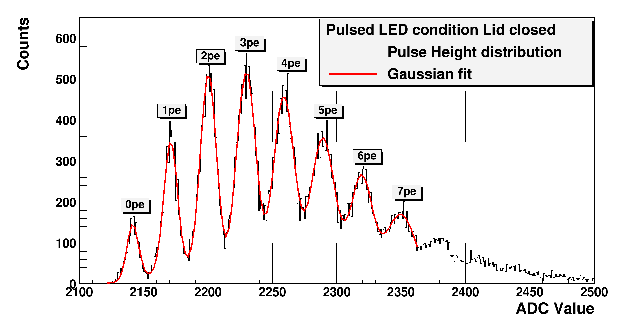
\includegraphics[angle=0, width=12.5cm]{PIXEL60_PDM20_HG_DICEMBRE_2018.eps}
\vspace{0.5cm}
\caption{ Pulse height spectrum at a fixed temperature of 15$^\circ$C
and $V_{0}$=57 V for a camera pixel, during a FOC run in the HG electronics chain. 
The black curve represents the distribution of the peak detector output and the red curve shows the corresponding
multiple peaks Gaussian fit.}
\label{fig1}
\end{figure*}

\textbf{\textit{Dark counts runs}} are acquired
when the lids of the camera are closed.
The light-tight lid, in addition to protecting the FSC, it ensures that no light
can enter it when the lid is latched shut. In this way, it is possible to read out
the pulse height of all the signals pixel for each triggered dark event.
In absence of light, using the Low Gain electronics chain, the majority of events are 
contained in one peak position, named pedestal. 
It, that does not vary with temperature(\cite{Impiombato2016}), is considered as offset electronics chain in the analysis of cherenkov images for the astronomical
observations.
Each pulse height spectrum of the camera pixels, is fitted with a Gaussian function, allowing to obtain the exact peak position value in the ADC counts with the relative width (see Fig.~\ref{fig2}).





\begin{figure*}[h!!]
\centering
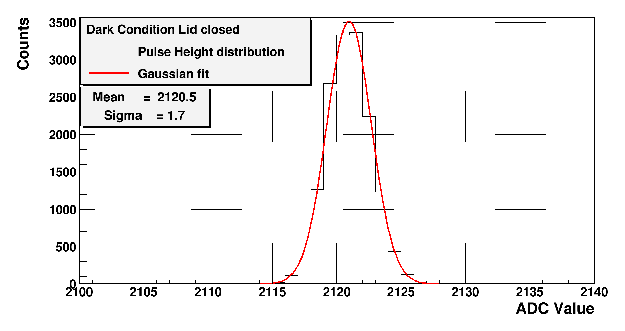
\includegraphics[angle=0, width=12cm]{PIXEL60_PDM20_LG_DICEMBRE_2018.eps}
\vspace{0.5cm}
\caption{ Single photo-electron peak spectrum for a camera pixel taken in peak detector mode in one of the Dark run listed in 
Table~\ref{table2}. The black curve represents the distribution of the peak detector
output and the red curve shows the corresponding Gaussian fit.}
\label{fig2}
\end{figure*}
\label{subs:skydata}





\begin{table*}[htbp!!]
\centering
\caption{ASTRI-Horn FOC/Dark runs}
\label{table2}
\begin{tabular}{lccc}
\hline\hline
Run ID & Starting Date & Run type      & Number of events \\
               & (year/month/day h:m:s)   \\
\hline     
1380 & 2018/12/01 20:59:18  &   Dark    & 15305      \\
1394 & 2018/12/02 20:01:09  &   FOC     & 60065     \\
1616 & 2019/02/28 12:37:02  &   Dark    & 50000     \\
1763 & 2019/03/23 20:01:21  &   FOC     & 120123    \\
  

\hline\hline
\end{tabular}
\end{table*}

\subsection{Open sky data} 
\label{subs:skydata}

Data used for the analysis refer to the period between December 2018 and March 2019 when the telescope was mainly involved in the Crab observation campaign. The list of the considered run ID is reported in Table~\ref{tab:obslog}; runs are split in several files, each containing a maximum of 50000 events, identified with a progressive number.
A selection was applied in order to avoid data affected by technical problems as instability in the PDM signals or fluctuation of the trigger rate. Moreover, intervals with bad atmospheric conditions 
(high humidity, low external temperature, cloudiness) were not considered as well as the periods when UVscope data are not available.

In each detected events we considered only the nine central PDM (11, 12, 13, 18, 19, 20, 25, 26, 27 in Fig.~\ref{fig: camera} ) taking into account the smaller UVscope FOV.  In addition, bad pixels and pixels imaging stars with a magnitude higher than …, coherently with the procedure adopted for UVscope data, are excluded from the analysis. The position of the stars in ASTRI-Horn FOV is computed from the correspondence with UVscope pixels derived from the variance method (Segreto et al 2019). 
The variance method was not used to identify stars because the relative data were not available in December and, for uniformity in the analysis, we decide to not use it either in March.  However, March variance data were used to cross-check the positions obtained from the correspondence with UVscope pixels.


\begin{table}[ht]
\label{tab:astrilog}
\caption{ASTRI-Horn observation log}
\centering
\begin{tabular}{lcccc}
\hline\hline
Observation ID & Starting Date & Exposure      & Number of events & pointing \\
               & (year/month/day h:m:s) & (s)  \\
\hline     
%https://www.overleaf.com/project/5e3005eb54e0d8000155a7ff

1429 & 2018/12/05 20:57:37  &   2094     & 31755 & Crab Off    \\
1430 & 2018/12/05 21:54:40  &   909      & 29808 & Fixed AltAzi Azi$=180°$ EleV. $=70°$    \\
1453 & 2018/12/07 20:06:11  &   6016     & 348442 & Crab Off    \\
1453 & 2018/12/07 20:06:11  &   6016     & 348442 & Crab Off    \\
1453 & 2018/12/07 20:06:11  &   6016     & 348442 & Crab Off    \\
1453 & 2018/12/07 20:06:11  &   6016     & 348442 & Crab Off    \\



1453 & 2018/12/07 20:06:11  &   6016     & 348442 & Crab Off    \\
1454 & 2018/12/07 22:09:16  &   4377     & 226651 &  Crab \\ %226650  \\
1455 & 2018/12/07 23:30:08  &   6243     & 412451 &  Crab \\ %412446    \\
1456 & 2018/12/08 01:24:48  &  8530     & 237318 & Crab Off \\ %  237186 \\
1457 & 2018/12/07 03:50:20  &  3509     & 126295 & Fixed ALtAzi\\ % 126264   \\
1464 & 2018/12/08 20:30:37 &  2255 & 97257 & Crab Off \\ %97251 \\  
1465 & 2018/12/08 21:17:34 &  9624 & 430245 & Crab\\ % 430222\\  
1466 & 2018/12/09 00:07:25 &  3161 & 251442 & Crab \\ %251418  
1467 & 2018/12/08 01:09:44 &  8959 & 243713 & Crab Off \\ %243399
1468 & 2018/12/08 03:40:11 &  1237 & 33168 &  Fixed AltAzi\\ %33126
1658 & 2019/03/05 18:13:58 &  112 & 1435 & Merak \\  
1659 & 2019/03/05 18:19:26 &  154 & 3149 & Zeta Tauri \\  
1660 & 2019/03/05 18:24:37 &  6224  & 419636 & Crab \\ %419631  
1661 & 2019/03/05 20:10:15 &  168 & 14389 & Zeta Tauri \\  
1662 & 2019/03/05 20:19:59 &  4008 & 198186 & Crab Off \\   
1663 & 2019/03/05 21:29:34 &  2337 & 165264 &  Fixed AltAzi \\  
1670 & 2019/03/06 18:08:27 &  628    &   8191      &  Merak\\
1671 & 2019/03/05 18:21:51 &  126        &   2412   & Zeta Tauri \\
1672 & 2019/03/05 18:25:56 &  5935    &   296073   &  Crab \\ %296046
1673 & 2019/03/05 20:06:58 &  183      &   3272     & Zeta Tauri\\ %3270
1674 & 2019/03/05 20:13:37 &  13812      &    152393 & Crab Off  \\ %152110     \\
%1466 & 2018/12/09 20:47:50 &  1218 & 50000 \\  

\hline\hline
\end{tabular}
\end{table}

Background pixels were identified applying the same double cut cleaning procedure used for the Cherenkov shower images. This procedure considers background pixels the ones that have a signal lower than a first threshold $S1$, or , if higher than $S1$, with none of the neighboring pixels with a signal higher that the second threshold $S2$. In our analysis, we adopted the values $S1$=6 and $S2$=12 used by Mineo et al. 2019 instead of higher values adopted for the analysis of Crab events (Lombarbi et al. 2018) to avoid muon signals.

For each event we then accumulated the distribution of the number of $p.e.$ in the background pixels. The curve obtained for the file 1473 of the run ID 000 is plotted in Fig.~\ref{fig:distr} as example. It is a distribution with a Gaussian shape in the central part and with long wings due to residual signals in the positive part and to … ???? in the negative one. 

The central part of the distribution is then fitted with a Gaussian whose $\sigma$ is the measure of the NSB fluctuations that, being a Poissonian signal, is linked to the absolute flux. The RMS values for December 9—10 observation night are plotted in Fig.~\ref{fig:rms} as function of time.

Finally, we plot the resulting values of $\sigma$ for each observing night in Fig.\ref{fig:sigma}  as a function of time. 


\subsection{Closed camera data} (Domenico)\\
The first step of the analysis chain is the camera calibration. 
It concerns the relative calibration 
of the pixels in the camera, i.e. the signal extraction and conversion into 
physical units, and the estimation of the level of statistical 
fluctuations of the pixel signals.
For the ASTRI-Horn, the signal waveforms are acquired with a 
sampling in peak detector mode, in order to obtain a pulse height distributions (PHD) for 
each physical pixel.
However the calibrated data must be expressed in term of 
photo-electrons(p.e.). Therefore the conversion factors from the maximum 
amplitude of the pulse to p.e. and from the integral of the pulse to p.e. 
must be known. 
The method to extract the conversion factor, also called gain, is to calculate the equivalent 
signal (maximum amplitude in ADC) for a single photon.
To do so, the ASTRI-Horn plans to have two types of low light level runs:\\
\textbf{\textit{FOC runs}} are acquired during the physics data taking.
In order to avoid that these events overlap with physics event, the light is flashed 
at a lower rate than the expected physics trigger rate. The light 
produced by the FOC must be uniform and should have an average of 
few p.e. per pixel. This allows to monitor continuously the gain of the 
electronics chain. Figure~\ref{fig1} shows the pulse height spectrum acquired in one of the FOC run listed in Table~\ref{table2} with a fixed voltage $V_{0}$= 57 V 
and a temperature of 15$^\circ$C for a camera pixel in the High Gain electronics chain. 
The distribution shown is the reconstructed maximum amplitude for all the 
recorded waveforms of a physical pixel. While the first peak is the pedestal, the following 
ones are the single and multiple p.e. contributions. The distance between 
the peaks allow to extract the conversion factor.\\
\begin{figure*}[ht!!]
\centering
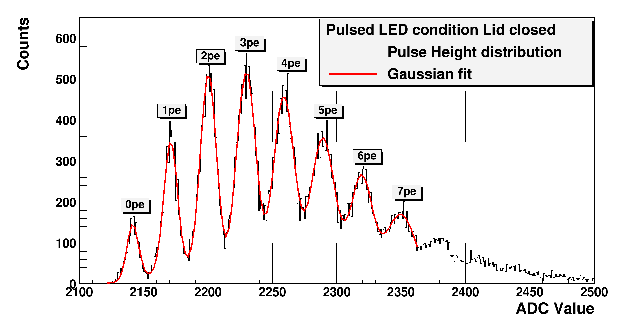
\includegraphics[angle=0, width=12.5cm]{PIXEL60_PDM20_HG_DICEMBRE_2018.eps}
\vspace{0.5cm}
\caption{ Pulse height spectrum at a fixed temperature of 15$^\circ$C
and $V_{0}$=57 V for a camera pixel, during a FOC run in the HG electronics chain. 
The black curve represents the distribution of the peak detector output and the red curve shows the corresponding
multiple peaks Gaussian fit.}
\label{fig1}
\end{figure*}

\textbf{\textit{Dark counts runs}} are acquired
when the lids of the camera are closed.
The light-tight lid, in addition to protecting the FSC, it ensures that no light
can enter it when the lid is latched shut. In this way, it is possible to read out
the pulse height of all the signals pixel for each triggered dark event.
In absence of light, using the Low Gain electronics chain, the majority of events are 
contained in one peak position, named pedestal. 
It, that does not vary with temperature(\cite{Impiombato2016}), is considered as offset electronics chain in the analysis of cherenkov images for the astronomical
observations.
Each pulse height spectrum of the camera pixels, is fitted with a Gaussian function, allowing to obtain the exact peak position value in the ADC counts with the relative width (see Fig.~\ref{fig2}).





\begin{figure*}[h!!]
\centering
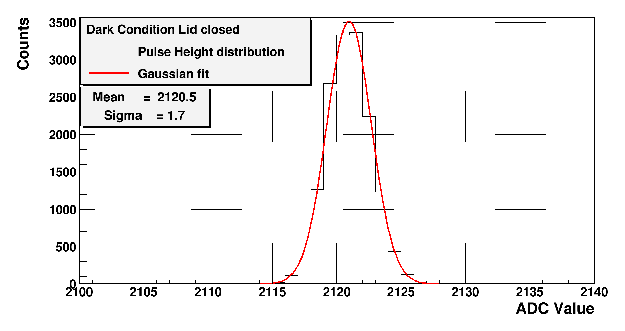
\includegraphics[angle=0, width=12cm]{PIXEL60_PDM20_LG_DICEMBRE_2018.eps}
\vspace{0.5cm}
\caption{ Single photo-electron peak spectrum for a camera pixel taken in peak detector mode in one of the Dark run listed in 
Table~\ref{table2}. The black curve represents the distribution of the peak detector
output and the red curve shows the corresponding Gaussian fit.}
\label{fig2}
\end{figure*}
\label{subs:skydata}





\begin{table*}[htbp!!]
\centering
\caption{ASTRI-Horn FOC/Dark runs}
\label{table2}
\begin{tabular}{lccc}
\hline\hline
Run ID & Starting Date & Run type      & Number of events \\
               & (year/month/day h:m:s)   \\
\hline     
1380 & 2018/12/01 20:59:18  &   Dark    & 15305      \\
1394 & 2018/12/02 20:01:09  &   FOC     & 60065     \\
1616 & 2019/02/28 12:37:02  &   Dark    & 50000     \\
1763 & 2019/03/23 20:01:21  &   FOC     & 120123    \\
  

\hline\hline
\end{tabular}
\end{table*}
